%! Author = Leonhard Gahr <leonhard.gahr@gmail.com>
%! Date = 25/04/21
%! Info = Studienarbeit

\chapter{Einleitung}
\enquote{Der digitale Wandel ist in vollem Gange. Die technologischen Entwicklungen sind rasant und verändern die Art, wie wir uns informieren, wie wir kommunizieren, wie wir konsumieren – kurz: wie wir leben. Diesen Wandel wollen wir als Chance begreifen, mehr Wohlstand und mehr Lebensqualität für die Bürgerinnen und Bürger zu schaffen, und ihn gleichzeitig sozialverträglich und im Einklang mit unseren Grundwerten gestalten.} \cite{bmwi2021}

So schreibt das \gls{bmwi} auf seiner Homepage einleitend zu den Zukunftsstrategien der Bundesregierung zur Ausgestaltung des Digitalen Wandels. Die im November 2018 verabschiedete Umsetzungsstrategie \enquote{Digitalisierung gestalten}\footcite{bundesregierung2020} soll die Grundlage dafür bilden, dass alle Bürger die Chancen der Digitalisierung nutzen und sich aktiv mit Kompetenz und Risikobewusstsein am digitalen Transformationsprozess unserer Gesellschaft beteiligen können. 

Nahezu gleichzeitig wurde im September 2018 das 7. Energieforschungsprogramm der Bundesregierung „Innovationen für die Energiewende“ auf den Weg gebracht, welches mithelfen soll, die energiepolitischen Ziele 
\begin{itemize}
    \itemsep0em
    \item[--] Reduktion des Primärenergieverbrauchs (Basis 2008) um 50\%
    \item[--] Treibhausgasreduktion (Basis 1990) um 80\%
    \item[--] Stromverbrauch (Basis 2008) um 25\%
    \item[--] Strom aus Erneuerbaren: Anteil 80\%
\end{itemize}
bis zum Jahre 2050 zu realisieren.

Dies soll u.a. durch intensive betriebliche und institutionelle Forschungsaktivitäten der Energieverbrauchssektoren „Gebäude und Quartier“, „Industrie, Gewerbe, Handel und Dienstleistungen“ sowie „Mobilität und Verkehr“ erreicht werden. Hierfür werden im Rahmen der Energieforschung im Jahre 2019 82,9 Mio. € Fördermittel für 854 laufende Vorhaben aus dem Bereich „Gebäude und Quartiere“ ausbezahlt \cite[Seite~80]{ptj2019}. Damit kommt der Effektivitätserhöhung im Gebäudebereich eine hohe Bedeutung zum Erreichen der Klimaziele zu, immerhin verbraucht dieser Bereich gut 30\% des bundesdeutschen Endenergieverbrauchs (2515 TWh in 2019)

\begin{figure}[htbp]
    \centering
    \fbox{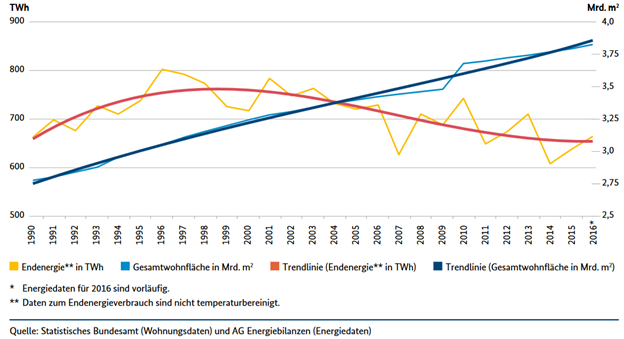
\includegraphics[width=\textwidth]{img/energieverbrauch}}
    \caption{\label{fig-energy}Energieverbrauch der Privaten Haushalte für Wohnen: Entwicklung des Endenergieverbrauchs insgesamt, sowie der Gesamtwohnfläche}
\end{figure}

Digitalisierung und Energieeffizienz, passen diese beiden Programme denn überhaupt zusammen? Lässt sich die schnelllebige digitale Welt mit den extrem langlebigen Erneuerungszyklen beim Gebäudebestand koppeln um sowohl den individuellen Anforderungen an Komforterhöhung und Energie -Effizienzsteigerung bei der Gebäudenutzung gerecht zu werden?

Mit der vorliegenden Arbeit wird eine Methodik erarbeitet, die marktverfügbare smarte Geräte mit den \gls{TGA} -Schnittstellen der Wohngebäude koppeln kann und durch Beobachten und Auswerten des spezifischen Bewohnerverhaltens den Gebäudebetrieb in einem möglichst globalen energetischen (Wärme, Strom) und ressourcenbezogenen (Wasser, Gas, Öl) Verbrauchsminimum ermöglicht, sowie den Komfort in der Nutzung jener Geräte erhöht.  
Das Energieeinsparpotential ist aufgrund des großen Multiplikators von 15,928 Mio. Einfamilienhäusern\footcite{statistica2020} immens. So verbraucht ein durchschnittlicher 4-Personenhaushalt ca. 4.000 kWh Strom pro Jahr und durchschnittlich 22.400 kWh Wärmeenergie pro Jahr. Dabei verteilt sich der Energieverbrauch auf die einzelnen Verbrauchscluster gemäß \cref{fig:energieverbrauch}:

\begin{figure}[htbp]
    \centering
    \fbox{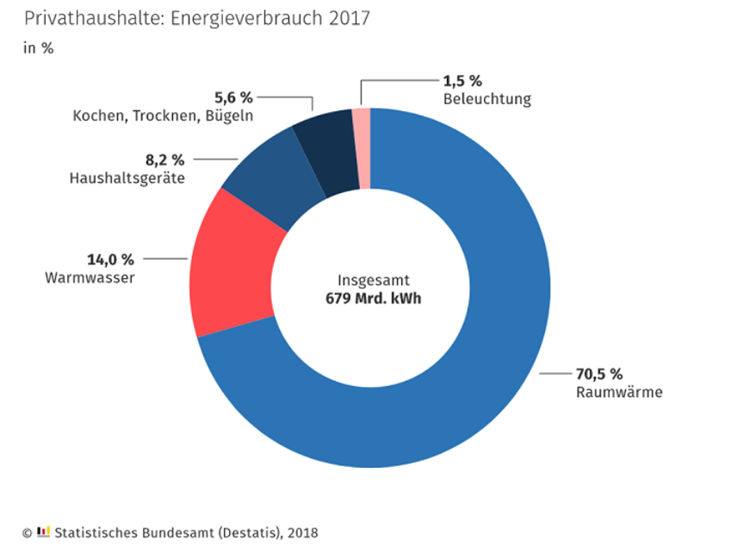
\includegraphics[width=\textwidth]{img/energieverbrauch_anteilig}}
    \caption{\label{fig:energieverbrauch}Energieverbrauch Privathaushalte 2017}
    \source{\url{https://www.effizienzhaus-online.de/energieverbrauch-haus/}}
\end{figure}